% !TEX root = template.tex
\section{Results}
\label{sec:results}
During the training part we have tried to use both validation accuracy and validation loss as metrics to understand which epoch provides the best model, no noticeable differences were found with the overall accuracy.

Looking at the training epochs, Fig.~\ref{fig:trainingPlot}, we can see that the weak models converge quickly: even if we trained our model for 100 epochs, we can see how the convergence is reached in less than 50 epochs.

\begin{figure}[h]
\begin{center}
        \centering
        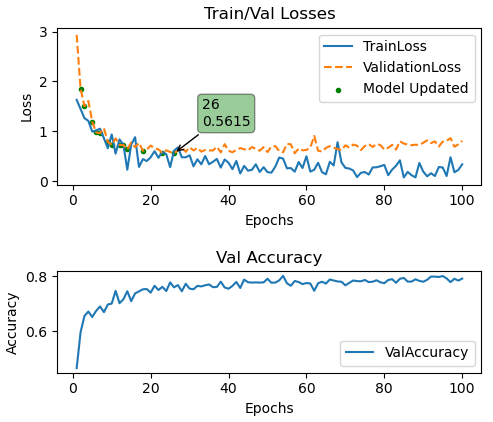
\includegraphics[width=0.5\textwidth]{resources/training_m0.png}
        \caption{Training of the Weak Model M0. The upper part shows losses on train and validation sets, and the lower part shows the accuracy on validation}
        \label{fig:trainingPlot}
    \end{center}
\end{figure}

The results for the weak models fulfils our expectations, and the loss and accuracy on the validation are:

\begin{minipage}{\textwidth}

\begin{verbatim}

  loss: 0.5616 - accuracy: 0.83 
  loss: 0.8126 - accuracy: 0.83
  loss: 0.4826 - accuracy: 0.85
  loss: 0.3892 - accuracy: 0.87
  loss: 0.4627 - accuracy: 0.86
  
\end{verbatim}
\end{minipage}
\\
    %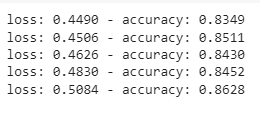
\includegraphics{results3.PNG}
At the end, the ensembled model shows an overall accuracy of 0.88.

The results show us how the bagging of 5 models increase slightly the overall accuracy of final decision. 

\begin{table}[h]
	\centering
	\caption{Weak models and ensembled model precisions on the classes}
	\label{tab:precisions}
	\begin{tabular}{|c||c|c|c|c|c||c|}
		\hline
		Class & M0 & M1 & M2 & M3 & M4 & EN\\
		\hline
		\hline
  
            0:bathtub      & \textbf{0.98} & \textbf{0.98} & 0.94 & 0.97 & 0.93 & \textbf{0.98}\\\hline
            1:bed          & 0.92 & 0.90 & 0.92 & \textbf{0.96} & 0.94 & 0.94\\\hline
            2:chair        & 0.96 & 0.91 & \textbf{0.98} & 0.94 & 0.96 & 0.97\\\hline
            3:desk         & 0.62 & 0.67 & \textbf{0.80} & 0.75 & 0.65 & 0.78\\\hline
            4:dresser      & 0.74 & 0.73 & 0.71 & \textbf{0.83} & 0.74 & 0.77\\\hline
            5:monitor      & 0.94 & \textbf{0.97} & \textbf{0.97} & 0.96 & \textbf{0.97} & 0.96\\\hline
            6:night\_stand & 0.71 & 0.75 & 0.75 & \textbf{0.81} & 0.67 & 0.75\\\hline
            7:sofa         & 0.88 & 0.76 & 0.81 & 0.87 & \textbf{0.90} & 0.88\\\hline
            8:table        & 0.67 & 0.77 & 0.73 & 0.76 & \textbf{0.81} & 0.78\\\hline
            9:toilet       & \textbf{0.99} & 0.90 & 0.95 & 0.91 & 0.98 & 0.97\\\hline
		\hline
            ACCURACY       & 0.83 & 0.83 & 0.85 & 0.87 & 0.86 & \textbf{0.88}\\\hline

  %           0:bathtub      & 0.98 & 0.98 & 0.94 & 0.97 & 0.93 & 0.98\\\hline
  %           1:bed          & 0.92 & 0.90 & 0.92 & 0.96 & 0.94 & 0.94\\\hline
  %           2:chair        & 0.96 & 0.91 & 0.98 & 0.94 & 0.96 & 0.97\\\hline
  %           3:desk         & 0.62 & 0.67 & 0.80 & 0.75 & 0.65 & 0.78\\\hline
  %           4:dresser      & 0.74 & 0.73 & 0.71 & 0.83 & 0.74 & 0.77\\\hline
  %           5:monitor      & 0.94 & 0.97 & 0.97 & 0.96 & 0.97 & 0.96\\\hline
  %           6:night\_stand & 0.71 & 0.75 & 0.75 & 0.81 & 0.67 & 0.75\\\hline
  %           7:sofa         & 0.88 & 0.76 & 0.81 & 0.87 & 0.90 & 0.88\\\hline
  %           8:table        & 0.67 & 0.77 & 0.73 & 0.76 & 0.81 & 0.78\\\hline
  %           9:toilet       & 0.99 & 0.90 & 0.95 & 0.91 & 0.98 & 0.97\\\hline
  %           \hline
  %           ACCURACY       & 0.83 & 0.83 & 0.85 & 0.87 & 0.86 & 0.88\\\hline
	\end{tabular}
\end{table}

Upon exploring the results, see Tab.~\ref{tab:precisions} for reference, we saw that each trained model had difficulties with different object categories, validating our hypothesis that weak models learn different things. 

All the trained models has difficulties in classifying similar shaped object like \textit{desk}s, \textit{dresser}s, \textit{night\_stand}s, and \textit{table}s. Models usually classify \textit{desk}s as \textit{table}s and \textit{night\_stand}s as \textit{dresser}s. 
This is also valid for the ensembled model, as it has to combine the results of the weaker models, and Fig.~\ref{fig:confusion_matrix} confirms it.
Fig.~\ref{fig:confusion_matrix} shows a matrix representing the predictions of the ensembled model on the test set. The matrix is almost diagonal, which signals that most of the predicted models are correctly classified.

\begin{figure}[h]
\begin{center}
        \centering
        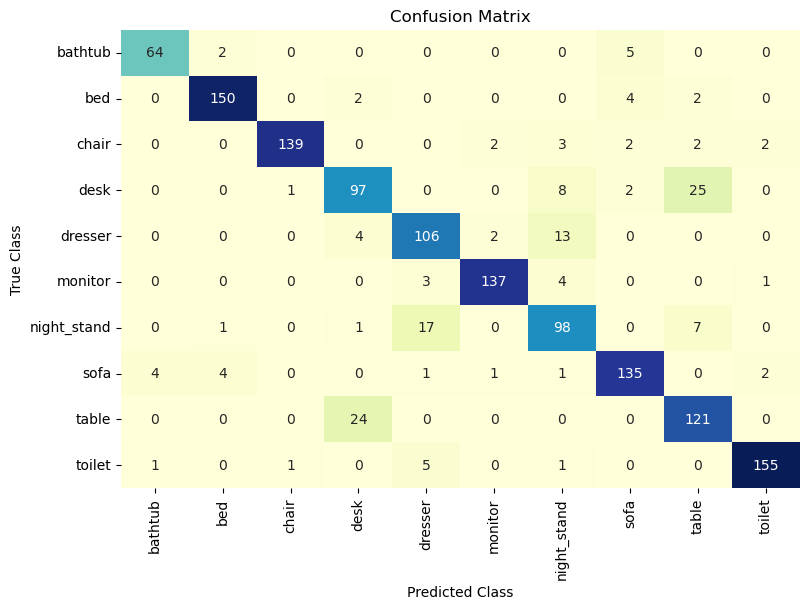
\includegraphics[width=0.5\textwidth]{resources/confusion_matrix_ensemble.png}
        \caption{Confusion Matrix of the Ensembled Model}
        \label{fig:confusion_matrix}
    \end{center}
\end{figure}

As a benchmark, we tried to train the baseline CNN model with only aligned 3D Objects resulting in an accuracy of 0.90. As expected, the rotations bring a higher level of complexity in classifying the objects. Rotations also make it harder for the models to overfit the dataset.